\section{Data Preprocessing}
Data preprocessing is a critical step to ensure the quality and effectiveness of summarization models. It is essential to clean and filter the data accurately.\\
Several cleaning and filtering operations were performed on the dataset to ensure data quality and consistency during model training.\\
Below are the steps carried out in this phase:
\subsection{Text Cleaning}
The following preprocessing steps were applied:

\begin{enumerate}
    \item \textbf{Lowercasing the text}
    \begin{itemize}
        \item This conversion ensures uniformity in the text, preventing the same word from being considered different solely due to the presence of uppercase letters.\\For example, "Home", "HOME", and "home" are treated as the same word, reducing vocabulary dimensionality and improving training efficiency.
    \end{itemize}

    \item \textbf{Removing HTML tags}
    \begin{itemize}
        \item Reviews may contain residual HTML tags from the original web format. 
        These elements do not contribute to the semantic meaning of the text and may interfere with model learning, so they are removed.
    \end{itemize}

    \item \textbf{Expanding contractions}
    \begin{itemize}
        \item Contractions in the English language (such as "don't", "I'm", "we're") are expanded to their full forms ("do not", "I am", "we are").\\
        This process aims to standardize and ensure consistency throughout the text and helps the model better capture semantic relationships by eliminating unnecessary variations of the same expression.
    \end{itemize}

    \item \textbf{Removing possessive forms ('s)}
    \begin{itemize}
        \item The possessive form in English does not substantially alter the meaning of the sentence for summarization purposes.\\
        Its removal simplifies the text and further reduces vocabulary size, allowing the model to focus on key concepts.
    \end{itemize}

    \item \textbf{Removing text in parentheses}
    \begin{itemize}
        \item Text within parentheses often contains supplementary information that is not generally essential for the summary.\\
        Removal helps maintain focus on the main information in the review.
    \end{itemize}

    \item \textbf{Removing punctuation and special characters}
    \begin{itemize}
        \item Punctuation and special characters, while important for human readability, can introduce noise into model training.\\
        Their removal simplifies the text while preserving the essential semantic content needed for summary generation.
    \end{itemize}

    \item \textbf{Removing stopwords}
    \begin{itemize}
        \item Stopwords are very common words (such as "the", "is", "at", "which") that appear frequently but carry little semantic meaning.\\
        Their removal significantly reduces the dimensionality of the problem without losing crucial information for the summary, allowing the model to focus on the most meaningful words.
    \end{itemize}

    \item \textbf{Removing very short words}
    \begin{itemize}
        \item Very short words (usually one or two letters) often do not contribute to the meaning of the text.\\
        Their removal helps further reduce noise in the data, keeping only the most significant terms for analysis.
    \end{itemize}
\end{enumerate}

\subsection{Data Filtering}
After a statistical analysis of the dataset, the following constraints were applied:
\begin{itemize}
    \item Maximum length of reviews: 30 words
    \item Maximum length of summaries: 8 words
\end{itemize}

These limits were determined through statistical analysis of the length distributions in the dataset, as shown in Figure \ref{fig:dataset_length_distribuition}.
\begin{figure}[H]
    \centering
    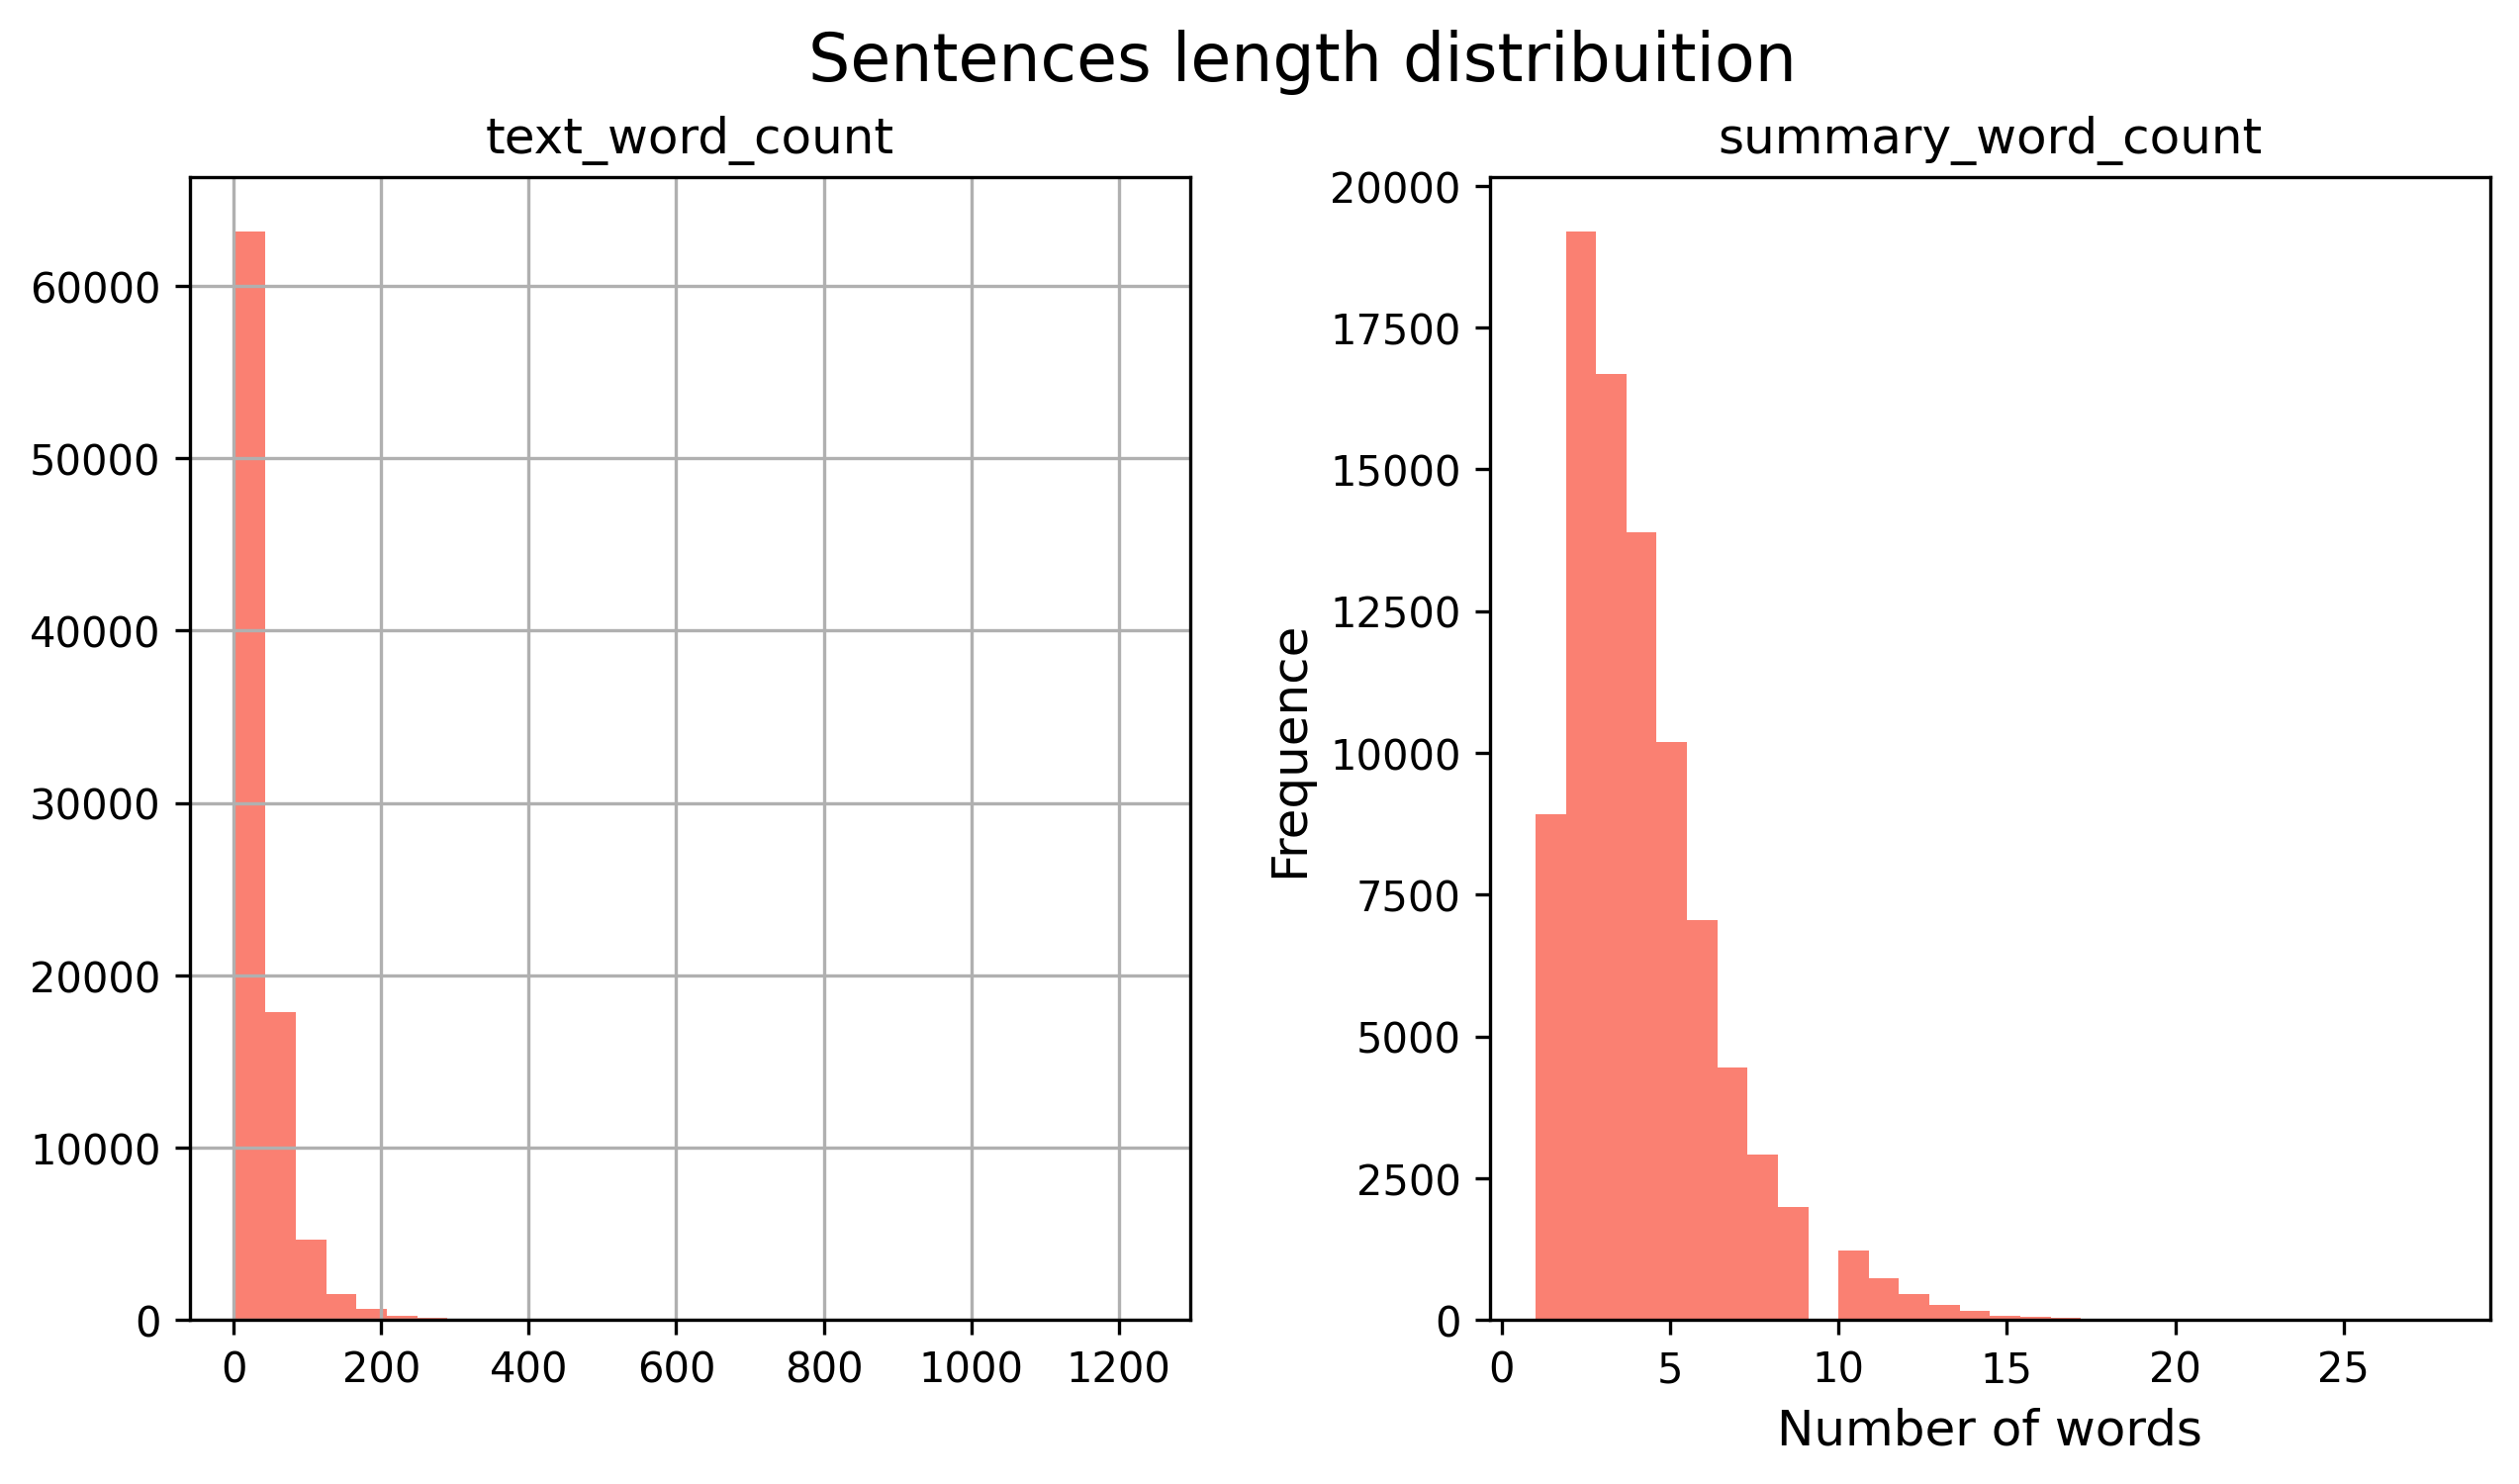
\includegraphics[width=1\textwidth]{media/dataset_length_distribuition.png}
    \caption{On the left, the distribution of review lengths; on the right, the distribution of summary lengths}
    \label{fig:dataset_length_distribuition}
\end{figure}
Indeed, as can be seen from the two graphs, most reviews and summaries have lengths below the established limits, so these constraints allow for the retention of most of the dataset's data.

\subsection{Tokenization and Special Tokens}
To prepare the data for the models, I added the special tokens \texttt{"sostok"} and \texttt{"eostok"} to indicate the beginning and end of a sequence, facilitating tokenization and the training phase.\\
Additionally, I performed tokenization separately for reviews (input text) and summaries (output text) to ensure that the model can correctly learn the relationship between the two.
The two tokenizers are used to create the vocabulary for reviews and for summaries, allowing the conversion of texts into sequences of tokens.
